\chapter{Analyzing Audio Fingerprint}
\label{chp:analyzing} 

\section{CPU microinstruction setup}\label{sec:ch4_cpu_microinstruction_setup}
Before jumping at RSA key extraction, we want to verify that we are able to distinguish the audio fingerprint created by a computer repreating microinstructions. 
The idea is that repeating the same microinstruction over a period of time should produce a distinct audio fingerprint identifying that microinstruction. 
However, the fingerprint is heavily dependent on the targeted hardware configuration. 
For this reason, we got our hands on a Lenovo ThinkPad T60p laptop computer, which is fairly similar in terms of how the computer is built and what hardware is used, so we expect there to be a higher probability of observing the suggested phenomenons using this computer.
\todo{Get a Evo N200!!!, see section 3 in paper}

The laptop is running Linux Mint 17, and starting out we compile and run the following program to repeat the microinstructions 

\begin{lstlisting}[language=C, caption={Simple Microinstruction Loop}]
// see http://en.wikibooks.org/wiki/LaTeX/Source_Code_Listings
// \lstinputlisting[language=C]{loop_operations.c}
int main() {
	return 0;
}
\end{lstlisting}


\section{Looking at microinstructions}\label{sec:ch4_microinstructions}
Initially, we did were repeating the instructions \( NOP\), \( MUL\) and \( ADD\).
As previously mentioned, our sampling rate of \( 96kHz\) limited our ability to observe the frequency spectrum of the signal to frequencies less than \( 48kHz\).
In this interval we were unable to emirically distinguish the spectrums representing the intervals in time corresponding to the different instructions.
This is not surprising, as the original research shows that there is no obvious visible difference in the frequency response of these three instructions in the frequency range we are observing, even on the laptop with the most rich acoustic leakage.\todo{Refer to Figure 7 in the long paper} 

On the other hand, the paper suggests that looking at HLT compared to NOP and MEM should produce a significant distinguisability even in the frequency range we are working with, given that the instructions are executed on an Evo N200 laptop.
The problem with this is that the HLT instruction must be run in kernel space.
For that reason we choose to focus on distinguishing between MEM and NOP, to be able to keep utilizing our simple setup, and avoid the troubles of kernel space programming.

\section{analyze.c}\label{sec:ch4_analyse}


\section{Results}\label{sec:ch4_results}


\begin{figure}[h]
    \centering
    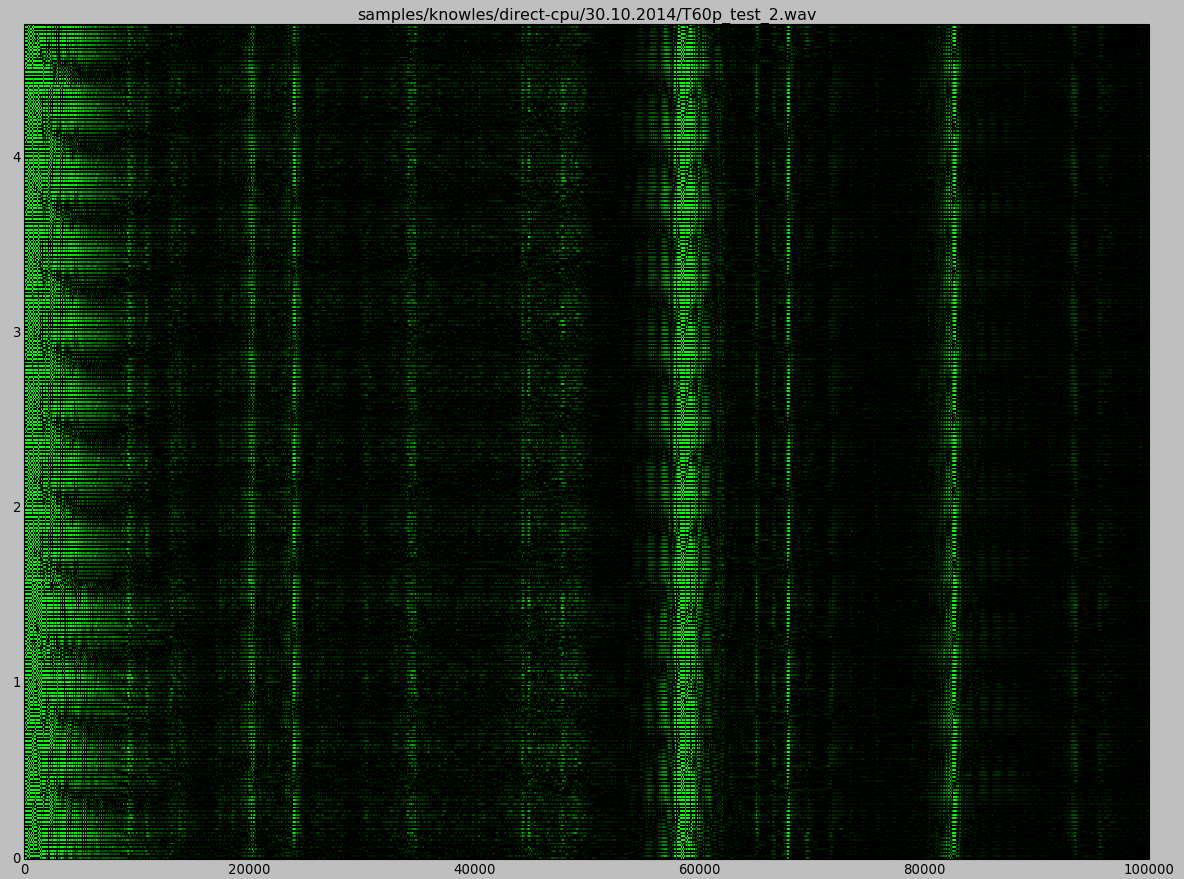
\includegraphics[width=5in]{T60p_eps_micro.png}
    \caption{Acoustic recording (5 sec, 0-100kHz) of the Lenovo T60p when performing NOP, MEM, MUL and ADD with external power supply. The recording was made using the Knowles Ultrasonic SPU0410LR5H~\cite{knowles_spec} microphone with the NI myDAQ. }
    \label{fig:T60p_eps_micr}
\end{figure}

\begin{figure}[h]
    \centering
    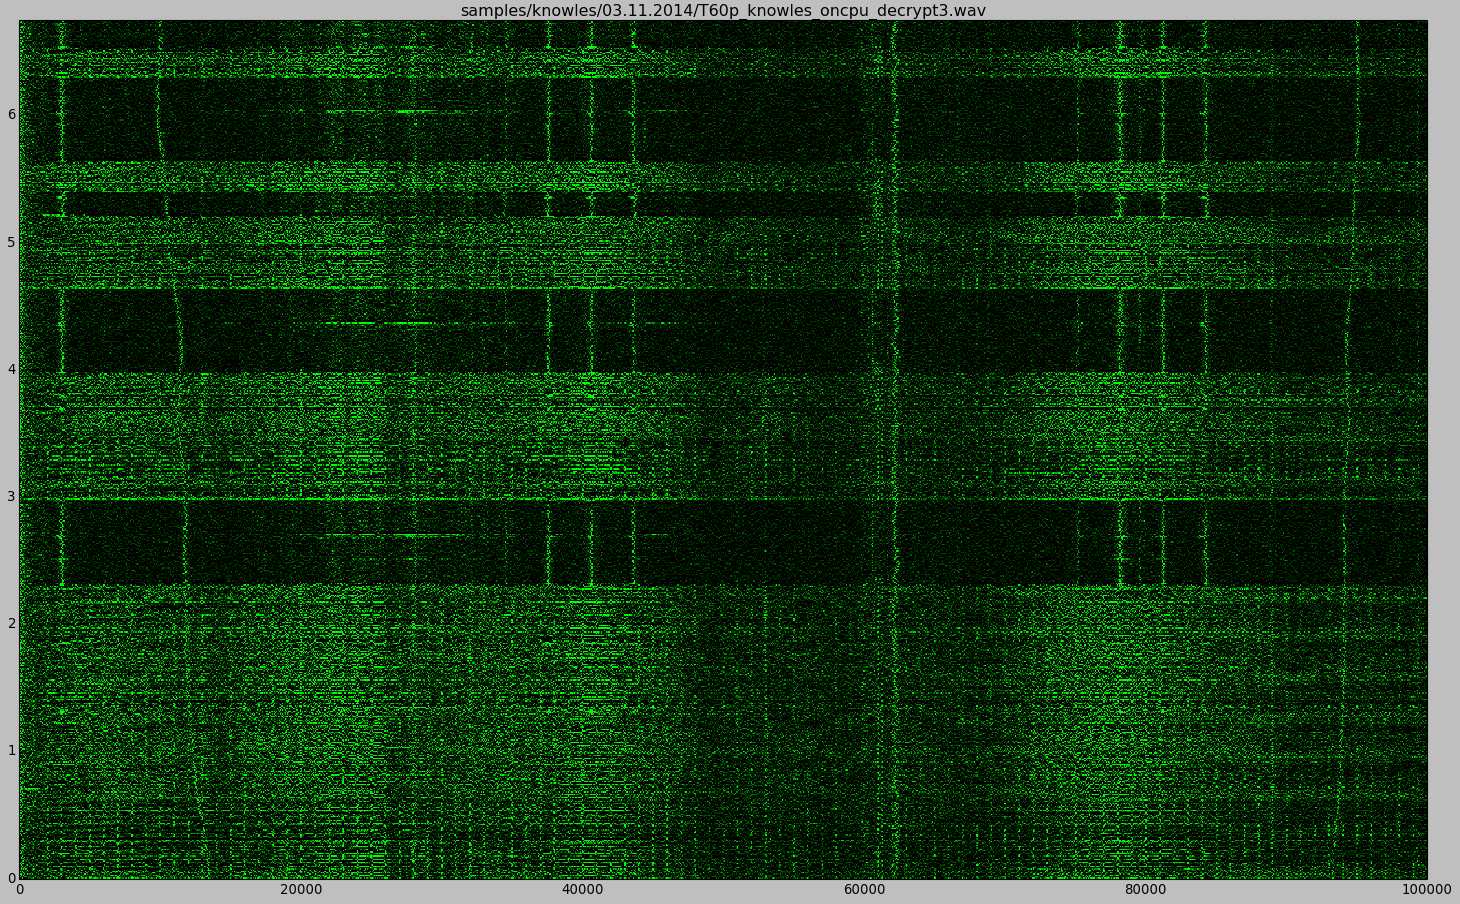
\includegraphics[width=5in]{T60p_battery_decrypt.png}
    \caption{Acoustic recording (7 sec, 0-100kHz) of the Lenovo T60p when performing 3 times RSA 4096-bit key decryption with internal power supply (i.e. battery) and 1 second sleep inbetween. The recording was made using the Knowles Ultrasonic SPU0410LR5H~\cite{knowles_spec} microphone with the NI myDAQ. }
    \label{fig:T60p_battery_decrypt}
\end{figure}

\begin{figure}[h]
    \centering
    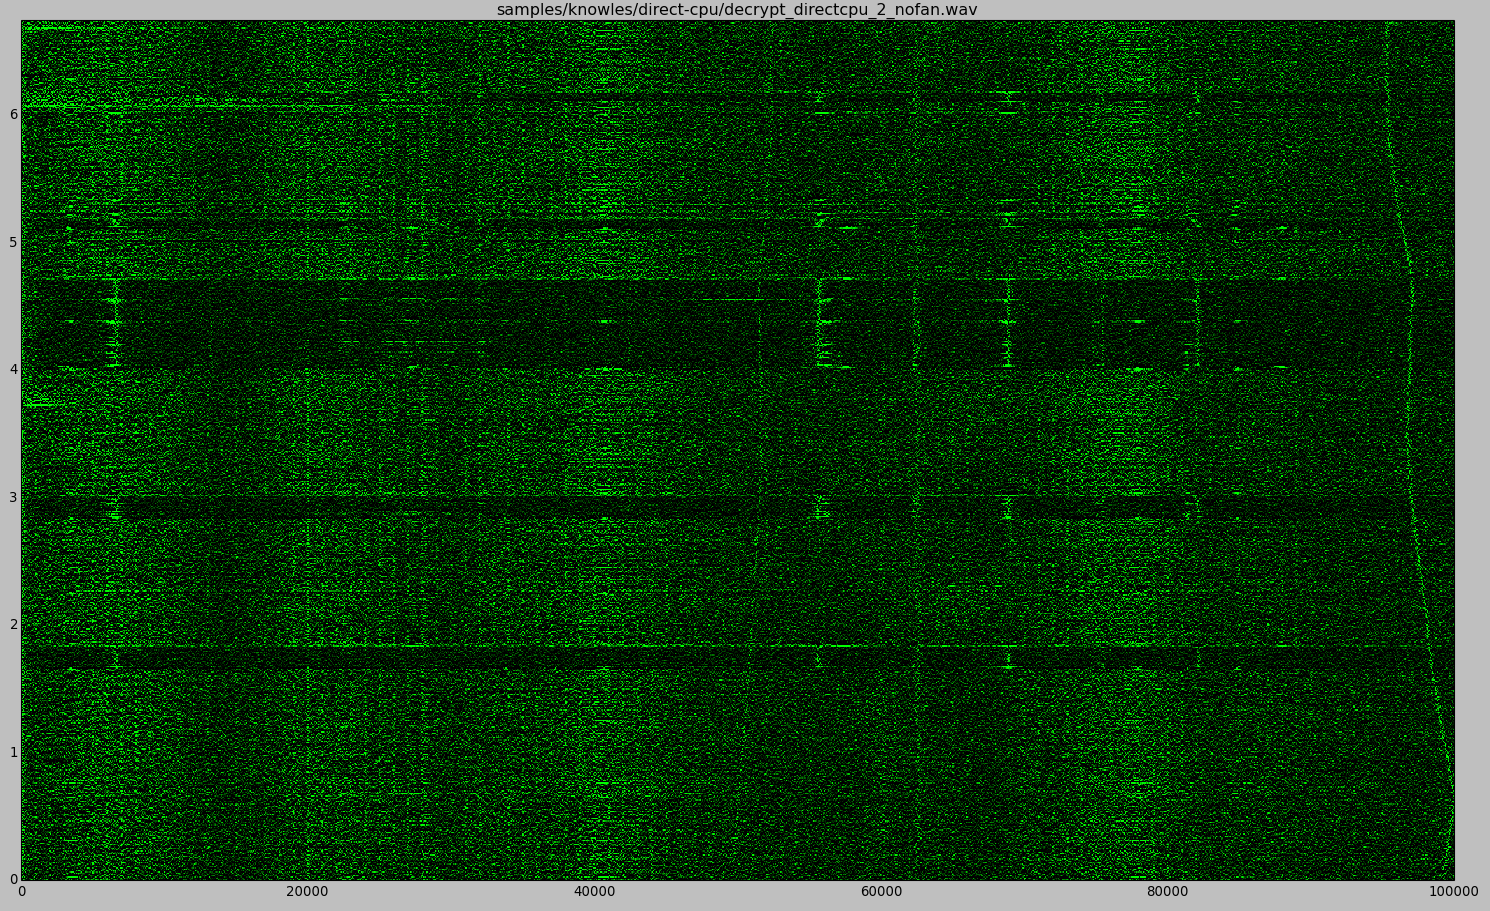
\includegraphics[width=5in]{T60p_battery_decrypt_2.png}
    \caption{Acoustic recording (7 sec, 0-100kHz) of the Lenovo T60p when performing 6 times RSA 4096-bit key decryption with internal power supply (i.e. battery) and 1 second sleep between the 1st and 2nd, 2nd and 3rd, then 4 subsequence decryptions. The recording was made using the Knowles Ultrasonic SPU0410LR5H~\cite{knowles_spec} microphone with the NI myDAQ. }
    \label{fig:T60p_battery_decrypt_2}
\end{figure}

\begin{figure}[h]
    \centering
    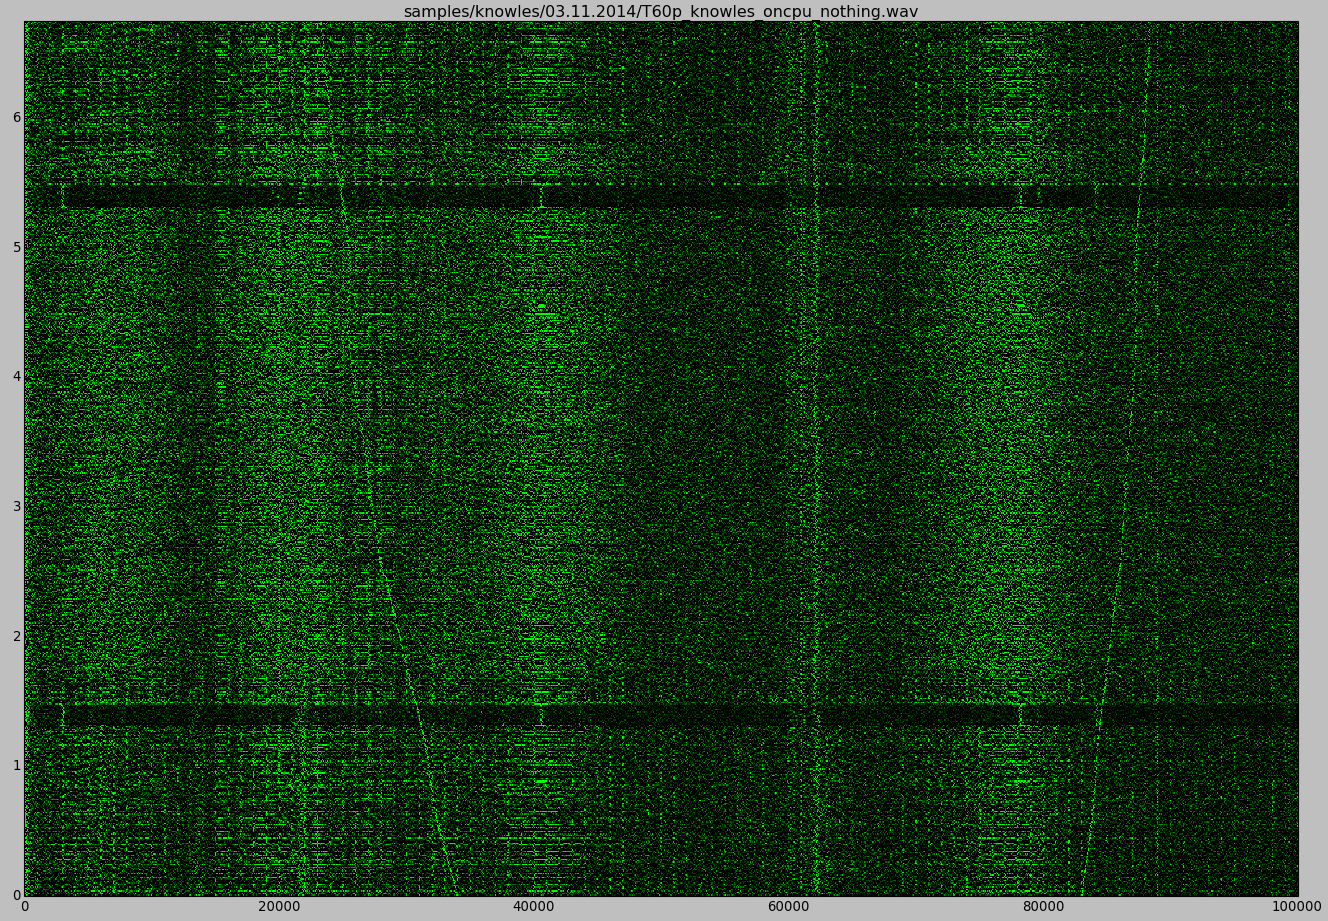
\includegraphics[width=5in]{T60p_battery_nothing.png}
    \caption{Acoustic recording (7 sec, 0-100kHz) of the Lenovo T60p when idle with internal power supply (i.e. battery). The recording was made using the Knowles Ultrasonic SPU0410LR5H~\cite{knowles_spec} microphone with the NI myDAQ. }
    \label{fig:T60p_battery_nothing}
\end{figure}